\documentclass[12pt,a4paper]{article}
\usepackage[utf8]{inputenc}
\usepackage[magyar]{babel}
\usepackage[T1]{fontenc}
\usepackage{amsmath}
\usepackage{amsfonts}
\usepackage{amssymb}
\usepackage{graphicx}
\author{Petrányi Bálint}\usepackage[pdfusetitle]{hyperref}
\usepackage{titling}
\usepackage[x11names]{xcolor}
\usepackage{xparse}
\usepackage{tcolorbox}
\usepackage{graphicx}
\usepackage{enumerate}
\graphicspath{ {./images/} }

\hypersetup{
    colorlinks,
    citecolor=black,
    filecolor=black,
    linkcolor=black,
    urlcolor=black
}

\date{\today}
\author{Petrányi Bálint}
\title{%
	\textbf{Analzízis Alkalmazásai.} \\
	\textbf{Programtervező informatikus A. szakirány} \\
	RöpZh Tételek\\
	\large 2023-2024. tanév 2. félév
}
\newcommand{\norm}[1]{\lVert #1 \rVert}
\newcommand{\R}{\mathbb{R}}
\newcommand{\CR}{\mathcal{R}}
\newcommand{\N}{\mathbb{N}}
\newcommand{\CD}{\mathcal{D}}
\newcommand{\CL}{\mathcal{L}}
\newcommand{\CM}{\mathcal{M}}
\newcommand{\m}{\varrho}
\newcommand{\f}{\varphi}
\newcommand{\fn}{f_n}
\newcommand{\KH}[1]{\text{KH}(#1)}
\newcommand{\tf}{\tilde{\f}}
\newcommand{\met}[1]{\m \left( #1 \right)}
\newcommand{\bb}[1]{\left( #1 \right)}
\newcounter{count}
%\setcounter{count}{#3} #1_{\thecount},\setcounter{count}{\numexpr\thecount+1} #1_{\thecount}, \ldots, #2_{#4} 
\NewDocumentCommand{\ton}{ O{1} O{n} o o } {\IfValueTF{#3}{\IfValueTF{#4}{\setcounter{count}{#3} #1_{\thecount},\setcounter{count}{\numexpr\thecount+1} #1_{\thecount}, \ldots, #2_{#4}}{\setcounter{count}{#3} #1_{\thecount},\setcounter{count}{\numexpr\thecount+1} #1_{\thecount}, \ldots, #2_{n}}}{ #1, #1, \ldots, #2 }}
\newcommand{\oneton}{1,2,\ldots ,n}
\newcommand{\nrom}[1]{\lVert #1 \rVert}
\newcommand{\angels}[1]{\langle #1 \rangle}
\newcommand{\abs}[1]{\left| #1 \right|}
\newcommand{\braces}[1]{\left\lbrace #1 \right\rbrace}
\newcommand{\boxes}[1]{\left[ #1 \right]}


\newtheorem{tet}{Tétel}[section]
\tcolorboxenvironment{tet}{
  colback=blue!10!white,
  boxrule=0pt,
  boxsep=1pt,
  left=2pt,right=2pt,top=2pt,bottom=2pt,
  oversize=2pt,
  sharp corners,
  before skip=\topsep,
  after skip=\topsep,
}

\newtheorem{defi}{Definíció}[section]
\tcolorboxenvironment{defi}{
  colback=green!15!white,
  boxrule=0pt,
  boxsep=1pt,
  left=2pt,right=2pt,top=2pt,bottom=2pt,
  oversize=2pt,
  sharp corners,
  before skip=\topsep,
  after skip=\topsep,
}

\tcolorboxenvironment{proof}{
  colback=red!30!white,
  boxrule=0pt,
  boxsep=1pt,
  left=2pt,right=2pt,top=2pt,bottom=2pt,
  oversize=2pt,
  sharp corners,
  before skip=\topsep,
  after skip=\topsep,
}

\begin{document}
\maketitle
\tableofcontents
\newpage
\section{week}
\subsection{Mikor mondjuk, hogy a $\f$ függvény az $f(x, y) = 0$ egyenletnek egy implicit megoldása?}
\begin{defi}
Legyen $f \in \R^2 \rightarrow \R$ egy adott függvény. Ha létezik olyan $I \subset \R$ nyílt intervallum és $\f : I \rightarrow \R$ függvény, hogy 
\[
f(x,\f(x)) = 0 \quad (\forall x \in I)
\]
akkor azt mondjuk, hogy a $\f$ függvény az $f(x, y) = 0$ implicit alakban van megadva
\end{defi}
\subsection{Hogyan szól az egyváltozós implicitfüggvény-tétel?}
\begin{tet}[Egyváltozós implicitfüggvény-tétel.]
Legyen $\Omega \in \R^2$ nyílt halmaz és $f : \Omega \rightarrow \R$. Tegyük fel, hogy
\begin{enumerate}
\item[(a)] $f$  folytonosan deriválható $\Omega$-n
\item[(b)] az $(a,b) \in \Omega$ pontban $f(a,b) = 0 $ és $\partial_2 f(a,b) \neq 0$
\end{enumerate}
Ekkor:
\begin{enumerate}
\item Van olyan $K(a) =: U$ és $K(b) =: V$ környezet $\R$-ben, hogy minden $x \in U$ ponthoz létezik egyetlen $\f(x) \in V$, amelyre $f(x, \f(x)) = 0$
\item Az így definiált $\f : U \rightarrow V$ függvény folytonosan deriválható $U$-n, továbbá $\forall x \in U$-ra  $\partial_2 f(x,\f(x)) \neq 0$ és
\end{enumerate}
\[
\f'(x) = - \frac{\partial_1 f (x,\f(x))}{\partial_2 f(x,\f(x))}
\]
\end{tet}
\subsection{Igaz-e a következő állítás? \textit{"Az implicitfüggvény-tétel egy explicit előállítást ad az $f(x, y) = 0$ egyenlet implicit megoldására."} A válaszát indokolja meg!}
Nem igaz

Világos, hogy $\f(a) = b$. A $\f$ függvényt az $f(x, \f(x)) = 0 \; \; (x \in U)$ egyenlőség "implicit" módon definiálja. Innen származik a tétel neve.
A tétel csak a $\f$ implicit függvény létezéséről szól, ezt a függvényt általában nem tudjuk explicit képlettel előállítani. Ennek ellenére a $\f'(x)$ deriváltat ki tudjuk számítani, ha ismerjük a $\f(x)$ függvényértéket.
\subsection{A deriválási szabályok alapján hogyan vezethető le az $f(x, \f(x)) = 0 \; (x \in U)$ egyenlőségből az implicit megoldás deriváltjára vonatkozó összefüggést az $U$ környezetben?}
\[
F(x) := f(x,\f(x)) \quad (x \in U)
\]
Mivel $\forall x \in U $  esetén $F(x) = 0$, ezért $F'(x) = 0$. Az összetett függvény deriválási szabálya szerint
\begin{align*}
0 = F'(x) = \partial_1 f (x, \f(x)) &\cdot 1 + \partial_2 f(x,\f(x)) \cdot \f'(x) \quad (x\in U) \\
\text{ezért } \forall x \in U \text{ pontban:} \\
\f'(x) &= - \frac{\partial_1 f (x,\f(x))}{\partial_2 f(x,\f(x))}
\end{align*}
\subsection{Mit jelent az, hogy egy $\R^n \rightarrow \R^n$ típusú függvény lokálisan invertálható?}
\begin{tet}[Lokális invertálhatóság.]
Legyen $I \subset \R$ nyílt intervallum és $f : I \rightarrow \R$.

T.f.h. $f \in C^1(I)$ és egy $a \in I$ pontban $f'(a) \neq 0$

Ekkor $f$ az $a$-ban lokálisan invertálható, azaz $\exists U := K(a)$ és $V:= f[U]$ nyílt halmaz, hogy az  $f_{\mid_U} : U \rightarrow V$ függvény bijekció, ezért invertálható. Az $f_{\mid_U}^{-1}$ lokális inverz folytonosan deriválható $V$-n, és
\[
(f^{-1})' (y) = \frac{1}{f'(f^{-1}(y))} \quad (y \in V)
\]
\end{tet}
\subsection{Igaz-e, hogy minden $\R^2 \rightarrow \R^2$ típusú, folytonos és lokálisan invertálható függvény globálisan is invertálható? A válaszát indokolja meg!}
Nem igaz\\
Például az 
\[
f(x,y) := (e^x \cos y, e^x \sin y) \quad ((x,y)\in \R^2)
\]
folytonos függvény a sík minden $\pi$-nél kisebb sugarú körlapján injektív, de globálisan nem injektív, hiszen
\[
f(x,y+2\pi) = f(x,y) \quad (\forall (x,y)\in \R^2)
\]
\subsection{Hogyan szól az inverzfüggvény-tétel?}
\begin{tet}[Inverzfüggvény-tétel.]
Legyen $\Omega \subset \R^n \; (x\in\N)$  nyílt halmaz és $f: \Omega \rightarrow \R^n$. T.f.h
\begin{enumerate}
\item[(a)] $f$ folytonosan deriválható $\Omega$-n
\item[(b)] egy $a \in \Omega$ pontban $\det f'(a) \neq 0$
\end{enumerate}
Ekkor
\begin{enumerate}
\item $f$ lokálisan invertálható, azaz van olyan, az $a \in \Omega$ pontot tartalmazó $U$ nyílt halmaz, hogy ha $V := f[U]$, akkor az $f_{\mid_U} : U \rightarrow V$ függvény bijekció (következésképpen invertálható).
\item Az $\bb{f_{\mid_U}}^{-1}$ 
lokális inverz folytonosan deriválható $V$-n és
\[
\bb{f^{-1}}'(y) = \left[ f'(f^{-1}(y)) \right]^{-1} \quad (y \in V)
\]
\end{enumerate}
\end{tet}
\subsection{Igaz-e a következő állítás? \textit{"Az inverzfüggvény-tétel egy explicit előállítást ad bizonyos feltételeket teljesítő függvények inverzére."} A válaszát indokolja meg!}
Nem igaz

Az $f$ függvény explicit alakjának az ismeretében $f^{-1}$ helyettesítési értékeire általában nincs explicit képlet, viszont
\[
\bb{f^{-1}}'(y) = \left[ f'(f^{-1}(y)) \right]^{-1} \quad (y \in V)
\]
alapján a derivált helyettesítési értékei az $f'$ helyettesítési értékeinek felhasználásával már kiszámíthatók, ha ismerjük az inverz függvény értékét a megfelelő pontban
\newpage
\section{week}
\subsection{ Adja meg a két változós valós értékű $f$ függvény a $g = 0$-ra vonatkozó feltételes abszolút maximumának a fogalmát!}
\begin{defi}
Legyen $U \subset \R^2$ nyílt halmaz T.f.h $f,g: U \rightarrow \R $ adott függvények és
\[
H_g := \braces{z\in U \mid g(z) = 0} \neq 0
\]
$a \in H_g$ pontban \textbf{feltételes abszolút maximuma van} ha
\[
f(x) \leq f(a), \quad \forall x \in H_g \subset \CD_f = U
\]
\end{defi}

\subsection{Adja meg a két változós valós értékű $f$ függvény a $g = 0$-ra vonatkozó feltételes lokális maximumának a fogalmát}
\begin{defi}
Legyen $U \subset \R^2$ nyílt halmaz T.f.h $f,g: U \rightarrow \R $ adott függvények és
\[
H_g := \braces{z\in U \mid g(z) = 0} \neq 0
\]
$a \in H_g$ pontban \textbf{feltételes lokális maximuma van} ha
\[
\exists K(a) \subset U : f(x) \leq f(a), \quad \forall x \in K(a) \cap H_g 
\]
\end{defi}

\subsection{ Igaz-e, hogy egy feltételes abszolút maximum egyben feltételes lokális maximum? A válaszát indokolja meg!}
Igen
Mert van egy környezet amiben lokális maximum lesz

\subsection{Mondja ki az elsőrendű szükséges feltételről szóló tételt feltételes lokális szélsőértékekre!}
\textbf{Általános eset:}
\begin{tet}
T.f.h $n,m \in \N \; m < n, \; \emptyset \neq U \subset \R^n$ nyílt halmaz
\begin{enumerate}
\item[(a)] az $f : U \rightarrow \R $ és a $g = (g_1,\ldots , g_m) : U \rightarrow \R^m$ függvények folytonosan deriválhatók az $U$ halmazon
\item[(b)] az $a = (a_1, \ldots, a_n) \in U$ pontban az $f$ függvénynek a $g_1 = 0,\ldots ,g_m = 0$ feltételekre vonatkozóan feltételes lokális szélsőértéke van
\item[(c)] rang $\begin{bmatrix}
\partial_1 g_1(a) & \partial_2 g_1(a) & \ldots & \partial_n g_1(a) \\
\vdots & \vdots & \vdots & \vdots \\
\partial_1 g_m(a) & \partial_2 g_m(a) & \ldots & \partial_n g_m(a) 
\end{bmatrix} = 0 $
\end{enumerate}
Ekkor léteznek olyan $\lambda_1 , \ldots , \lambda_m \in \R$ (Lagrange-szorzók), hogy az
\[
\CL(x) := f(x) + \lambda_1 g_1 (x) + \ldots + \lambda_m g_m(x) \quad (x\in U)
\]
Lagrange-függvénynek $a = (a_1, \ldots , a_n)$ stacionárius pontja, azaz
\[
\CL' (a) = \boxes{\partial_1\CL(a), \ldots, \partial_n\CL(a)} = \boxes{0, \ldots ,0} = \theta_m \in \R^n
\]
\end{tet}

vagy 
\textbf{2 változos eset:}
\begin{tet}
T.f.h
\begin{enumerate}
\item[(a)] $U \subset \R^2 $ nyílt halmaz és az $f,g : U \to \R $ függvényeknek léteznek a parciális deriváltjaik és azok folytonosak az $U$ halmazon
\item[(b)] az $(x_0,y_0) \in U $ pontban az $f$ függvénynek a $g = 0$ feltételre vonatkozóan feltételes lokális szélsőértéke van
\item[(c)] $g' (x_0,y_0) = \bb{\partial_1 g(x_0,y_0),\partial_2 g(x_0,y_0)} \neq (0,0)$
\end{enumerate}
Ekkor van olyan $\lambda \in \R$ valós szám (ezt Lagrange-szorzónak
szokás nevezni), hogy az
\[
\CL(x,y) := f(x,y) + \lambda g(x,y) \quad \bb((x,y)\in U)
\]
Lagrange-függvénynek $(x_0, y_0)$ stacionárius pontja, azaz
\[
\CL'(x,y) = \bb{\partial_x\CL(x_0,y_0),\partial_y\CL(x_0,y_0)} = (0,0)
\]
\end{tet}
\subsection{Mondja ki a másodrendű elégséges feltételről szóló tételt feltételes lokális szélsőértékekre!}
\textbf{Általános eset:}
\begin{tet}
$n,m \in \N \; m < n, \; \emptyset \neq U \subset \R^n$ nyílt halmaz T.f.h:

$f,g_1,\ldots,g_m \in C^2$  és $\lambda_1,\ldots, \lambda_m \in \R$ olyan számok, valamint az $a \in U$ olyan pont, hogy az
\[
\CL := f+ \lambda_1g_1 + \ldots + \lambda_mg_m
\]
függvényre $\CL'(a) = \emptyset_n$ továbbá minden olyan $h \in \R^n, h \neq \subset_n$ vektorra, amelyre
\[
g_1'(a) \cdot h = 0, \; g_2'(a) \cdot h = 0, \ldots , \; g_m'(a) \cdot h = 0
\]
teljesül úgy, hogy 
\[
\angels{\CL''(a) \cdot h,h} > 0
\]
Ekkor az $f$ függvénynek a $g_1 = 0, \ldots , g_m = 0$ feltételek
mellett feltételes minimuma van az $a \in U $ pontban.
\end{tet}

vagy 
\textbf{2 változos eset:}
\begin{tet}
T.f.h
\begin{enumerate}
\item[(a)] $U \subset \R^2 $ nyílt halmaz és $f,g \in C^2(U,\R)$
\item[(b)] az $(x_0,y_0) \in U  $ pontban a $\lambda_0 \in \R $ számmal teljesül a szükséges feltétel. 
\end{enumerate}
Tekintsük ezzel a $\lambda_0$ számmal az
\[
\CL(x,y):= f(x,y) + \lambda_0g(x,y) \quad \bb{(x,y) \in U}
\]
Lagrange-függvényt. Legyen
\[
D(x_0,y_0;\lambda_0) := \det\begin{bmatrix}
0 & \partial_1g(x_0,y_0) & \partial_2g(x_0,y_0) \\
\partial_1g(x_0,y_0) & \partial_{11}\CL(x_0,y_0) & \partial_{12}\CL(x_0,y_0) \\
\partial_2g(x_0,y_0) & \partial_{21}\CL(x_0,y_0) & \partial_{22}\CL(x_0,y_0)
\end{bmatrix}
\]
(a mátrixot \textbf{kibővített Hesse-mátrixnak} szokás nevezni).
Ekkor:
\begin{enumerate}
\item ha $D(x_0,y_0;\lambda_0)> 0 \Leftarrow (x_0,y_0)$ feltételes lokális \textbf{maximumhely}
\item ha $D(x_0,y_0;\lambda_0)< 0 \Leftarrow (x_0,y_0)$ feltételes lokális \textbf{minimumhely}
\end{enumerate}
\end{tet}


\subsection{ Miért nem tudjuk általában alkalmazni a korábban megismert (nem feltételes) lokális szélsőértékek keresésére szolgáló módszert feltételes lokális szélsőértékek keresésére?}
Mert mindig feltettük, hogy a vizsgált pont az
értelmezési tartomány belső pontja. Könnyen látható azonban,
hogy a $H_g$ halmaznak nincs belső pontja.
\subsection{Milyen esetben tudjuk a kétváltozós függvényekre vonatkozó feltételes szélsőérték-problémát visszavezetni egy egyváltozós függvény szélsőérték-problémájára?}
T.f.h a feltételt megadó $g(x,y) = 0$ egyenletből (például) az $y$
kifejezhető az $x$ változó függvényeként, azaz $\exists \f \in \R \to \R $ függvény, amelyre $g(x,\f(x)) = 0 $

A $H_g = \braces{(x,y) \mid g(x,y) = 0} \subset \R^2$ halmaz tehát a $\f$ függvény garfikonja, ami "jó" esetben egy síkbeli "görbe". Az $f$ függvénynek a $H_g$ halmaz pontjaiban felvett értékeit a $h(x) := f(x,\f(x))$ alós-valós függvénnyel lehet kifejezni.

A kétváltozós függvényekre vonatkozó feltételes szélsőérték-problémát a szóban forgó esetben a $h$ egyváltozós függvény szélsőérték-problémájára lehet visszavezetni.
\subsection{Milyen esetekben és hogyan tudjuk a Weierstrass-tételt alkalmazni a feltételes abszolút szélsőrtékek keresésében?}
A feltételes abszolút szélsőértékhelyek megkeresése
egy "egyszerűbb" feladathoz vezethet, ha a
\[
H_g := \braces{x\in U \mid g(x) = 0}
\]
halmaz korlátos és zárt. Ebben az esetben a Weierstrass-tétel
garantálja a feltételes abszolút szélsőértékhelyek létezését, amelyek a Lagrange-függvény stacionárius pontjai lesznek.
\newpage
\section{week}
\subsection{Mit nevezünk szakaszonként sima útnak?}
\begin{defi}
A $\f : \boxes{a,b} \to \R^n$ függvény \textbf{szakaszonként sima
út}, ha
\begin{itemize}
\item $\f \in C \boxes{a,b}$
\item $\exists a = t_0 < t_ 1 < \ldots < t_m = b \; (m \in \N )$  olyan felosztása $\boxes{a,b}$-nek , amelyre tetszőleges $k = 0,1,\ldots,m-1$ index esetén $\f_{\vert_{\boxes{t_k,t_{k+1}}}}$ sima út
\end{itemize}
\end{defi}
\subsection{Mit nevezünk egy út ellentettjének?}
Egy $\f$ út $\tilde{\f}$ \textbf{ellentettjét} így definiáljuk:
\[
\tilde{\f} := \f(b+a-t) \quad (a \leq t \leq b)
\]
\subsection{Mit nevezünk az $u$ és $v$ pontokat összekötő szakasznak?}
Legyenek adottak az $u,v \in \R^n$  pontok, és legyen
\[
\f_{uv}(t) := u+t(v-u) \quad (0 \leq t \leq 1)
\]
Ekkor $\f_{uv}$ egy sima út, az $u$-t és $v$-t összekötő szakasz, amelynek a $\f_{uv}(0) = u$ a kezdőpontja, a $\f_{uv}(1) = v$ pedig a végpontja.
\subsection{Mikor mondjuk, hogy egy halmaz összefüggő, és mit nevezünk tartománynak?}
Azt mondjuk, hogy az $U \subset \R^n$ nyílt halmaz \textbf{összefüggő}, ha bármely két pontja összeköthető $U$-ban haladó töröttvonallal. Az összefüggő nyílt halmazokat röviden \textbf{tartománynak} nevezzük.
\subsection{Adja meg az $f$ függvény $\f$ útra vett vonalintegráljának fogalmát!}
\begin{defi}
T.f.h $U \subset \R^n \quad (n \in \R^n)$ tartomány, az $f: U \to  \R^n$ függvény folytonos, továbbá $\f : \boxes{a,b} \to  \R^n$ egy $U$-ban  haladó szakaszonként sima út. Ekkor az $f$ függvény $\f$ út vett vonalintegrálját így értelmezzük:
\[
\int\limits_\f f := \int\limits^b_a \angels{f \circ \f,\f'} = \int\limits^b_a \angels{f(\f(t)), \f'(t)} dt.
\]
\end{defi}
\subsection{Mondja ki a vonalintegrál utak egyesítéséről szóló állítás!}
\begin{tet}
Legyen $U \subset \R^n \quad (n\in \N)$ egy tartomány és t.f.h az $f,g : U \to \R^n$ függvények folytonosak.
Ha a $\f,\psi$ utak $U$-beliek és létezik a $\f \vee \psi $ egyesítésük, akkor
\[
\int\limits_{\f \vee \psi } f = \int\limits_\f f + \int\limits_\psi f
\]
\end{tet}
\subsection{Mondja ki a vonalintegrál utak ellentettjéről szóló állítás!}
\begin{tet}
Legyen $U \subset \R^n \quad (n\in \N)$ egy tartomány és t.f.h az $f,g : U \to \R^n$ függvények folytonosak.
bármilyen $U$-beli $\f$ út $\tilde{\f}$ ellentettjére
\[
\int\limits_{\tilde{\f}} f = -\int\limits_\f f 
\]
\end{tet}
\subsection{Adja meg egy $f$ vektormező primitív függvényének fogalmát!}
\begin{defi}
Legyen $U \subset \R^n$ egy tartomány és  $f = (f_1,\ldots,\f_n): U \to \R^n$ adott vektormező Azt mondjuk, hogy a $F : U \to \R$ függvény a $f$ függvény \textbf{primitív függvénye} ha $F$ differenciálható $U$-ban, és $F' = f$ azaz  ha minden $x \in U$ pontban
\[
F'(x) = \bb{\partial_1F(x),\ldots,\partial_nF(x)} = \bb{f_1(x),\ldots,f_n(x)}
\]
\end{defi}
\subsection{Mondja ki a Newton-Leibniz-tételt!}
\begin{tet}[Newton–Leibniz]
Legye $U \subset \R^n$ egy tartomány, és t.f.h. az $f : U \to \R^n$
folytonos függvénynek van primitív függvénye. Ekkor tetszőleges $U$-ban haladó $\f : [a, b] \to U$ szakaszonként sima út esetén a $f$ bármelyik $F$ primitív függvényével
\[
\int\limits_\f f = F(\f(b))-F(\f(a))
\]
\end{tet}
\subsection{Igaz-e a következő állítás? "Ha a folytonos $f : U \to \R^n$ függvénynek van primitív függvénye, akkor $f$ vonalintegráltjának értéke nulla tetszőleges $U$-ban haladó zárt úton" A válaszát indokolja meg!}
\newpage
\section{week}
\subsection{Mit jelent, hogy egy vonalintegrál független az úttól?}
\begin{tet}
Legyen $U \subset \R^n$ tartomány és $f = (f_1,\ldots,f_n): U \to \R^n$ folytonos függvény.

A vonalintegrál független az úttól. Ez azt jelenti, hogy ha az $U$-be
\[
\f : \boxes{a,b} \to U \quad \text{ és } \quad \psi : \boxes{c,d} \to U
\]
szakaszonként sima utak $\f(a) = \psi(c)$ és $\f(b) = \psi(d)$ azaz a $\f,\psi$ utak ugyanazt a kezdőpontot és végpontot köti össze $U$-ban, akkor
\[
\int\limits_\f f = \int\limits_\psi f
\]
\end{tet}
\subsection{Milyen állításokat ismer, amelyek ekvivalensek azzal, hogy minden vonalintegrál független az úttól?}
\begin{tet}
Legyen $U \subset \R^n$ tartomány és $f = (f_1,\ldots,f_n): U \to \R^n$ folytonos függvény.
\begin{enumerate}
\item A $f$-nek létezik primitív függvénye $U$-n, vagyis $\exists F : U \to \R$ differenciálható függvény, amelyre minden $x \in U$ pontban
\[
F'(x) = \bb{\partial_1F(x),\ldots,\partial_nF(x)} = \bb{f_(x),\ldots,f_n(x)}
\]
\item Minden $U$-ban haladó $\f : \boxes{a,b} \to U $ U szakaszonként sima zárt (az $\f(a) = \f(b)$) útra
\[
\oint\limits_\f f = 0
\]
\end{enumerate}
\end{tet}
\subsection{Mondja ki a tanult szükséges feltételt primitív függvény létezésére vonatkozóan!}
\begin{tet}[Szükséges feltétel primitív függvény létezésére]
Legye $U \subset \R^n$ tartomány és $f = \bb{f_1,\ldots,f_n} : U \to \R^n$ deriválható függvény. Ha $f$-nek létezik primitív függvénye $U$-n, akkor az $f'$ deriváltmátrix szimmetrikus, azaz minden $x \in U$ pontban
\[
\partial_if_j(x)=\partial_jf_i(x) \quad \bb{i,j = 1,2,\ldots,n}
\]
\end{tet}
\subsection{Igaz-e a következő állítás? "Minden $f : \R^2 \to \R^2$ folytonos függvénynek van primitív függvénye." A válaszát indokolja meg!}
Nem igaz
Például
\[
f(x,y) := \bb{-\frac{y}{x^2+y^2},\frac{x}{x^2+y^2}} \quad \bb{(0,0) \neq (x,y) \in \R^2}
\]
Ennek a függvénynek $\int\limits_\f f \neq 0$ Mivel $\f$ zárt út $\mathcal{D}_f$-ben ezért $f$-nek nincs primitív függvénye. Az az deriválható még sincs primitív függvénye
\subsection{Mondja ki a tanult elégséges feltételt primitív függvény létezésére vonatkozóan!}
\begin{tet}[Elégséges feltétel primitív függvény létezésére]
Tekintsük az $U \subset \R^n \quad (n\in \N)$ csillagtartományon értelmezett $f=\bb{f_1,\ldots,\f_n} : U \to \R^n$ folytonosan deriválható függvényt.
T.f.h $\forall x \in U$ esetén az $f'(x)$ deriváltmátrix szimmetrikus, azaz minden $x \in U$ pontban
\[
\partial_if_j(x)=\partial_jf_i(x) \quad \bb{i,j = 1,2,\ldots,n}
\]
Ekkor $f$-nek van primitív függvénye, azaz $\exists F: U \to \R$ differenciálható függvény, hogy $\forall i = 1,\ldots,n$ index esetén $\forall x \in U$ pontban $\partial_iF(x)=f_i(x)$ 
\end{tet}
\subsection{Adja meg egy $v$ vektormező divergenciájának fogalmát!}
\begin{defi}
A $v = \bb{v_1,v_2,v_3} : D \to \R^3 \; \bb{D \subset \R^3 \text{ tartomány} }$ deriválható vektormező $v'$ deriváltmátrixának főátlójában álló elemeinek összegét, azaz a
\[
\text{div } \textbf{v} := \partial_1v_1+\partial_2v_2 + \partial_3v_3 : D \to \R
\]
függvényt a $v$ vektormező \textbf{divergenciájának} nevezzük.
\end{defi}
\subsection{Adja meg egy $v$ vektormező rotációjának fogalmát!}
\begin{defi}
A $v = \bb{v_1,v_2,v_3} : D \to \R^3 \; \bb{ D \subset \R^3  \text{ tartomány} }$ deriválható vektormező \textbf{rotációjának} a 
\[
\text{rot } \textbf{v}:=\boxes{\partial_2V_3-\partial_3V_2 \;\; \partial_3V_1-\partial_1V_3 \;\; \partial_1V_2-\partial_2V_1}
\]
függvényt nevezzük.
\end{defi}
\subsection{Mondja ki a Green-tételt!}
\begin{tet}[Green-tétel]
T.f.h $\f : \boxes{0,1} \to \R^2$ pozitív irányítású, szakaszonként sima, egyszerű, zárt görbe, és $S \subset \R^2$ az általa határolt síkrész.
Legye $f \in \R^2 \to \R^2, S \subset \CD_f$ folytonosan differenciálható függvény. Ekkor
\[
\int\limits_{\partial S} f = \iint\limits_s (\partial_1f_2-\partial_2f_1)
\]
ahol $\partial S$ az $S$ határát jelöli és $\f$ a $\partial S$ egy paraméterezése.
\end{tet}
\newpage
\section{week}
\subsection{Mit nevezünk explicit elsőrendű közönséges differenciálegyenletnek? Fogalmazza meg pontosan, hogy milyen feladatot oldunk meg ebben az esetben!}
\begin{defi}
\textbf{Feladat}

\underline{Adott:} \begin{itemize}
\item $D \subset \R^2$ tartomány
\item $f : D \to \R $ folytonos függvény
\end{itemize}
\underline{Keresünk} olyan $I \subset R$ nyílt intervallumot és $\f : I \to R$ deriválható függvényt, amelyre igazak a következő állítások:
\begin{align*}
\bb{x,\f(x)} \in D \quad &\bb{\forall x \in I} \\
\f'(x) = f\bb{x,\f(x)} \quad &\bb{\forall x \in I}
\end{align*}
Ezt a feladatot explicit elsőrendű közönséges differenciálegyenletnek fogjuk nevezni.
\end{defi}
\subsection{Mit nevezünk az explicit elsőrendű közönséges differenciálegyenletre vonatkozó kezdetiérték problémának? Fogalmazza meg pontosan, hogy milyen feladatot oldunk meg ebben az esetben!}
\begin{defi}
Tekintsük az $y' = f \circ (id, y)$ differenciálegyenletet, ahol $f : D \to \R \; (D \subset \R^2$ tartomány) folytonos függvény. Legyen $(\tau, \xi) \in D$ egy tetszőleges pont. Keressünk olyan $I \subset \R$ nyílt intervallumot és $\f : I \to R$ függvényt, amelyre a következők teljesülnek:
\begin{itemize}
\item $\f$ az $y' = f \circ (id,y)$ d.e. megoldása $I$-n
\item $\tau \in I$
\item $\f(\tau) = \xi$ 
\end{itemize} 
Ezt a feladatot kezdetiérték-problémának nevezzük.
\end{defi}
\subsection{Mit állít a Cauchy Peano-féle egzisztenciatétel?}
\begin{tet}[A Cauchy–Peano-féle egzisztenciatétel]
T.f.h a $D \subset \R^2$ tartományon értelmezett $f: D \to \R$ függvény folytonos. Ekkor bármely $\bb{\tau,\xi} \in D$ esetén az 
\[
y' = f \circ \bb{id,y} \quad \; y(\tau) = \xi
\]
kezdetiérték-problémának van megoldása.
\end{tet}
\subsection{Mit jelent, hogy egy kezdetiérték-probléma globálisan egyértelműen oldható meg?}
\begin{defi}
Az $y' = f \circ \bb{id,y}, \; y(\tau) = \xi$ k.é.p \textbf{globálisan egyértelműen oldható meg}, ha létezik olyan $\tilde{I} \subset \R$ nyílt intervallum és olyan $\tilde{\f}: \tilde{I} \to \R$ megoldása a k.é.p.-nak, hogy annak bármely más megoldása $\tilde{\f}$ egy leszűkítése. Ebben az esetben
a $\tilde{\f}$ függvényt a k.é.p. teljes megoldásának nevezzük.
\end{defi}
\begin{tet}
Az $y' = f \circ \bb{id,y}, \; y(\tau) = \xi$ k.é.p globálisan egyértelműen oldható meg, akkor és csak akkor ha a k.é.p bármely $\f,\psi$ megoldására a
\[
\f(x) = \psi(x) \quad \bb{x \in \CD_\f \cap \CD_\psi}
\]
egyenlőség teljesül.
\end{tet}
\subsection{Mit jelent, hogy egy kezdetiérték-probléma lokálisan egyértelműen oldható meg?}
\begin{defi}
Az $y' = f \circ \bb{id,y}, \; y(\tau) = \xi$ k.é.p \textbf{lokálisan egyértelműen oldható meg}, vagy a megoldása \textbf{lokálisan egyértelmű}, ha a $\bb{\tau,\xi}$ pontnak létezik olyan $K(\tau,\xi) \subset \R \times \R$ környezete, hogy az $f$ függvényt erre leszűkítve a megfelelő k.é.p. már globálisan egyértelműen oldható meg.
\end{defi}
\subsection{Mondja ki a kezdetiérték-problémák globálisan és lokálisan egyértelmű megoldhatóságának a kapcsolatáról szóló tétel!}
\begin{tet}
Az $y' = f \circ \bb{id,y}, \; y(\tau) = \xi$ k.é.p minden $\bb{\tau,\xi} \in D$ esetén lokálisan egyértelműen oldható meg akkor minden k.é.p. megoldása globálisan is egyértelmű.
\end{tet}
\subsection{Mit nevezünk szétválasztható változójú differenciálegyenletnek? Fogalmazza meg pontosan, hogy milyen feladatot oldunk meg ebben az esetben!}
\begin{defi}
\textbf{Feladat}

\underline{Adott:} \begin{itemize}
\item $I,J \subset \R$ nyílt intervallum
\item $g:I \to \R$ és $h:J\to \R$ folytonos függvények
\end{itemize}
\underline{Keresünk} olyan $I_1 \subset I$ nyílt intervallumot és $\f : I_1 \to J$ függvényt, amelyre:
\[
\f'(x) = g(x) \cdot h(\f(x)) \quad (\forall x \in I_1)
\]
Ezt a feladatot szétválasztható változójú d.e.-nek nevezzük
\end{defi}
\subsection{Mit tud mondani a szétválasztható változójú differenciálegyenletre vonatkozó kezdetiérték problémák megoldhatóságát illetően?}
\newpage
\section{week}
\subsection{Mit nevezünk egzakt differenciálegyenletnek? Fogalmazza meg pontosan, hogy milyen feladatot oldunk meg ebben az esetben!}
\begin{defi}
Legyen adott $H \subset \R^2$ tartomány és a $g,h : H \to \R$ folytonos függvények. Tegyük fel még azt is, hogy $0 \notin \mathcal{R}_h$. Keresünk olyan $\f : \R \to \R$ differenciálható függvényt amelyre $\CD_\f$ nyílt intervallum $(x,\f(x)) \in H $ és:
\[
\f'(x) = -\frac{g(x,(\f(x)))}{h(x,\f(x))} \quad (x \in \CD_\f)
\]
Ezt a feladatot egzakt differenciálegyenletnek nevezzük, ha az
\[
\R^2 \supset H \ni (u,v) \mapsto (g(u,v),h(u,v)) \in \R^2
\]
függvénynek van primitív függvénye, azaz létezik olyan $F: H \to \R$ differenciálható függvény, amelyre az igaz, hogy
\[
\text{grad } F = (\partial_1F,\partial_2F) = (g,h)
\]
\end{defi}
\subsection{Milyen tételt ismer az egzaktság eldöntésére?}
\begin{tet}[Az egzaktság eldöntése.]
Legye $H \subset \R^2 $ csillagtartomány (pl. konvex halmaz). T.f.h. $g,h \in C^1 (H,\R)$ valamint $0 \notin \CR_h$ Ekkor a
\[
\frac{dy}{dx} = \frac{g(x,y)}{h(x,y)} \quad \bb{(x,y) \in H}
\] 
d.e. pontosan akkor egzakt d.e., ha
\[
\partial_2g(u,v) = \partial_1h(u,v) \quad \bb{\forall (u,v) \in H}
\]
\end{tet}
\subsection{Mit tud mondani az egzakt differenciálegyenletre vonatkozó kezdeti érték-probléma megoldhatóságáról és megoldása előállításáról?}
\begin{tet}[Az egzakt d.e. megoldásainak előállítása.]
Legyen $H \subset \R^2$ egy tetszőleges tartomány. T.f.h. $g,h \in C (H,\R)$ és $0 \notin \CR_h$. Ekkor minden $(\tau,\varepsilon) \in H $ esetén a
\[
\frac{dy}{dx} = - \frac{g(x,y)}{h(x,y)} \quad \bb{(x,y)\in H } \quad y(\tau) = \varepsilon
\]
kezdetiérték-probléma globálisan egyértelműen oldható meg. Ha $F : H \to \R $ jelöli a $(g,h) : H \to \R^2$ függvény egy primitív függvényét, akkor a $(\tau,\varepsilon)$ ponton átmenő $\tf$ teljes megoldásra az
\[
F(x,\tf(x)) = F(\tau,\varepsilon) \quad \bb{x \in CD_{\tf}}
\]
implicit egyenlet teljesül.
\end{tet}
\subsection{Mit nevezünk integráló tényezőnek?}
Előfordulhat hogy a
\[
g(x,y)dx + h(x,y)dy = 0
\]
d.e. nem egzakt, de egzakttá tehető, vagyis az egyenlet egzakt lesz, ha megszorozzuk egy alkalmas pl. pozitív $\mu \in \R^2 \to \R $ függvénnyel, amelyet integráló tényezőnek vagy multiplikátornak szokás nevezni
\subsection{Mit nevezünk elsőrendű lineáris differenciálegyenletnek? Fogalmazza meg pontosan,hogy milyen feladatot oldunk meg ebben az esetben!}
\begin{defi}
Legyen $I \subset \R$ nyílt intervallum, és t.f.h. $f,g : I \to \R$ folytonos függvények. Az 
\[
y'(x)+ f(x)\cdot y(x) = g(x) \quad \bb{x \in I} \text{ vagy } y' + f \cdot y = g
\]
feladatot elsőrendű lineáris d.e.-nek nevezzük.
\end{defi}
\subsection{Milyen alakban írható fel egy elsőrendű inhomogén lineáris differenciálegyenlet általános megoldása bizonyos homogén-inhomogén megoldások ismeretében?}

\subsection{Mit nevezünk Bernoulli-féle differenciálegyenletnek? Fogalmazza meg pontosan, hogy milyen feladatot oldunk meg ebben az esetben!}
\begin{defi}
Legyen $I \in \R$ nyílt intervallum. T.f.h. $f, g \in C (I,\R)$ és $\alpha \in \R \setminus \braces{0,1}$ Ekkor az:
\[
y' + f \cdot y = g \cdot y^{\alpha} \quad \bb{y > 0}
\]
feladatot Bernoulli-féle d.e.-nek nevezzük.
\end{defi}
\subsection{Írja fel az explicit elsőrendű közönséges differenciálegyenletre vonatkozó kezdetiérték-problémát integrálegyenlet alakjában!}

\subsection{Mit állít a Picard Lindelöf-féle egzisztencia- és unicitástétel?}
\begin{tet}
Legyen $n \in \N, D \subset \R \times \R^n$ egy tartomány és $(\tau,\varepsilon) \in D$ teszőleges. Tegyük fel, hogy
\begin{enumerate}
\item az $f: D \to \R^n$ függvény folytonos $D$-n,
\item az $f$ függvény a $(\tau,\varepsilon)$ pontban a második változójában lokális Lipschitz-feltételnek tesz eleget, azaz
\begin{align*}
\exists K (\tau,\varepsilon) \subset D \subset \R \times \R^n \; \text{ és } \; \exists L:=L_{(\tau,\varepsilon)} > 0 \; \text{ hogy} \\
\norm{f(x,u)-f(x,v)} \leq L\norm{u-v} \quad \bb{(x,u),(x,v) \in K(\tau,\varepsilon)} 
\end{align*}
\end{enumerate} 
Ekkor az $y' = f \circ (id,y),\; y(\tau)= \varepsilon$ kezdetiérték-problémának létezik megoldása, és az lokálisan (következésképpen globálisan is) egyértelmű. 
\end{tet}
\subsection{Mit jelent, hogy az explicit elsörendü közönséges differenciálegyenletre vonatkozó kezdetiérték-problémának egy megoldása határtól határig halad egy tartományban!}
\begin{defi}
Legyen $f: D \to \R^n$, ahol $D \subset \R \times \R^n$. Azt mondjuk, hogy az $y' = f \circ (id,y) \; y(\tau)= \varepsilon$ k.é.p. $\f$ megoldása $D$-ben határtól határig halad, ha $D$ bármely $K$ kompakt részhalmazához vannak olyan $x_1,x_2 \in \CD_\f, x_1 < \tau < x_2$ pontok amellyel
\[
\bb{x_1,\f(x_1)} \notin K \; \text{ és } \;  \bb{x_2,\f(x_2)} \notin K
\]
\end{defi}
\newpage
\section{week}
\subsection{Mit nevezünk elsőrendű lineáris differenciálegyenlet-rendszernek? Fogalmazza meg pontosan, hogy milyen feladatot oldunk meg ebben az esetben!}
\begin{defi}
Legyen $n \in \N, I \subset \R $ nyílt intervallum, és t.f.h. az
\[
A : I \to \R^{n \times n} \quad \text{ és a } \quad b: I \to \R^n
\]
adott folytonos függvények. Ekkor az
\[
y'(x) = A(x) \cdot y(x) + b(x) \quad \bb{x \in I} \quad \text{ vagy } \quad y' = A \cdot y + b
\]
feladatot elsőrendű lineáris differenciálegyenlet-rendszernek (röviden lineáris d.e.r.) nevezzük.
\end{defi}
\subsection{Mit tudunk mondani egy elsőrendű lineáris differenciálegyenlet-rendszerre vonatkozó kezdetiérték-probléma megoldhatóságáról?}
\begin{tet}
Az (LKEP) k.é.p. minden $\tau \in I$ és $\varepsilon \in \R^n$ esetén globálisan egyértelműen oldható meg, és a teljes megoldás értelmezési tartománya az egész $I$ intervallum.
\end{tet}
\subsection{Mit nevezünk alaprendszernek elsőrendű lineáris differenciálegyenlet-rendszerek esetén?}
\begin{tet}
Az $\mathcal{M}_h$ lineáris térnek egy
\[
\f^{(k)} = \bb{\f_1^{(k)},\f_2^{(k)},\ldots,\f_n^{(k)}} \quad  \bb{k= 1,2,\ldots,n}
\]
bázisát az $y' = A \cdot y$ homogén d.e.r. egy alaprendszerének nevezzük
\end{tet}
\subsection{Mit nevezünk alapmátrixnak elsőrendű lineáris differenciálegyenlet-rendszerek esetén?}
\begin{tet}
Az $\mathcal{M}_h$ lineáris térnek az alaprendszereiből mint oszlopvektorokból képzett
\[
\Phi := \boxes{\f^{(1)} \; \f^{(2)} \; \ldots \; \f^{(n)}} = \begin{bmatrix}
\f_1^{(1)} & \f_1^{(2)} & \ldots & \f_1^{(n)} \\
\f_1^{(2)} & \f_2^{(2)} & \ldots & \f_2^{(n)} \\
\vdots & \vdots & \vdots & \vdots \\
\f_n^{(1)} & \f_n^{(2)} & \ldots & \f_n^{(n)}
\end{bmatrix}
\]
mátrixfüggvényt az egyenlet egy alapmátrixának nevezzük
\end{tet}
\subsection{Mit nevezünk egy megoldásrendszer Wronski-féle determinánsának elsőrendű lineáris differenciálegyenlet-rendszerek esetén?}
\begin{tet}
Az $\mathcal{M}_h$ lineáris térnek és ahol $\Phi$ az $y' = A \cdot y$ homogén lineáris d.e.r. egy alapmátrixa
\[
W(x) := \det \Phi(x) \quad \bb{x \in I}
\]
képlettel definiált $W$ függvény a megoldásrendszer Wronski-féle determinánsa.
\end{tet}
\subsection{Milyen jellegzetes tulajdonsága van egy alaprendszer Wronski-féle determinánsának?}
Nagyon nem vagyok ebben biztos:
\begin{tet}
Legyen $\f^{(1)},\f^{(2)},\ldots,\f^{(n)}$ az $y' = A \cdot y$ homogén d.e.r. egy alaprendszere és $\Phi$ egy alapmátrixa. Ekkor a $\Phi : I \to \R^{n \times n}$ mátrixfüggvény a homogén egyenletnek akkor és csak akkor alapmátrixa, ha valamilyen $x_0 \in I $ esetén 
\[
W(x_0) := \det \Phi(x_0) \neq 0
\]
\end{tet}
\subsection{Milyen alakban írható fel egy elsőrendű inhomogén lineáris differenciálegyenlet-rendszer általános megoldása bizonyos homogén-inhomogén megoldások ismeretében?}
\begin{tet}
Legyen $\psi_p$ az (IH) d.e.r egy ismert (ún. partikuláris) megoldása. Ekkor
\[
\CM_ih = \CM_h + \psi_p := \braces{\f + \psi_p \lvert \f \in \CM_h}
\]
Az inhomogén lineáris d.e.r. általános megoldása:
\[
\psi(x) = \Phi(x) \cdot c + \psi_p(x) \quad \bb{x \in I}
\]
alakú ahol $\Phi$ az $y' = A \cdot y$ homogén lineáris d.e.r. egy alapmátrixa és $c \in \R^{n \times 1 }$ tetszőleges oszlopvektor
\end{tet}

\subsection{Tegyük fel, hogy az elsőrendű állandó együtthatós lineáris differenciálegyenlet-rendszer együtthatókból álló $A \in \R^{n \times n}$ mátrixnak van $n$ számú különböző valós sajátértéke. Hogyan állíthatjuk elő egy alaprendszert ebben az esetben?}
Ilyenkor egy alaprendszere:
\[
\f^{i}(x) = e^{\lambda_{i}x} \cdot s^{(i)} \quad \bb{x \in \R, i = 1,2, \ldots, n}
\]
\newpage
\section{week}
\subsection{Mit nevezünk n-edrendű lineáris differenciálegyenletnek? Fogalmazza meg pontosan, hogy milyen feladatot oldunk meg ebben az esetben! }
\begin{defi}
Legyen $n \in \N, I \subset \R$ nyílt intervallum. T.f.h. az
\[
a_k : I \to \R \quad \bb{k = 0,1,\ldots,n-1} \quad \text{és a} \quad b : I \to \R
\]
adott folytonos függvények. Ekkor az
\[
\text{(nLDe)}
\begin{cases}
y^{(n)}(x) &+ a_{n-1}(x) \cdot y^{(n-1)}(x) + \ldots + \\
 &+ a_1(x) \cdot y'(x) + a_{0}(x) \cdot y(x) = b(x) \quad \bb{x \in I}
\end{cases}
\]
feladatot n-edrendű lineáris d.e.-nek nevezzük. Ha $b \equiv 0$, akkor homogén, az ellenkező esetben pedig inhomogén egyenletről beszélünk.
Most tehát olyan $J \subset I$ nyílt intervallumot és $\psi : J \to \R, \psi \in D^n$ függvényt keresünk, amelyre minden $x \in J$ helyen a
\[
\psi^{(n)}(x) + a_{n-1}(x) \cdot \psi^{(n-1)}(x) + \cdot + a_1(x) \cdot \psi'(x) + a_0(x) \cdot \psi(x) = b(x)
\]
egyenlőség teljesül. Ekkor $\psi$ a szóban forgó d.e. megoldása a $J$ intervallumon.
\end{defi}
\subsection{Fogalmazza meg pontosan mit értünk egy n-edrendű lineáris differenciálegyenletre vonatkoz ó kezdetiérték-problémán!}
\begin{defi}
Az nLde fogalmához és a megoldásán tull:
\[
\tau \in I \quad \text{hely és a} \quad \varepsilon := \bb{\varepsilon_0,\varepsilon_1,\ldots,\varepsilon_{n-1}} \in \R^n \text{vektor}  
\]
Ha a $\psi$ megoldástól azt is elvárjuk, hogy
\[
\tau \in J, \quad \psi(\tau)= \varepsilon_0, \psi'(\tau) = \varepsilon_1, \ldots , \psi^{(n-1)}(\tau) = \varepsilon_{n-1}
\]
akkor azt mondjuk, hogy a $\psi$ függvény a $J$ intervallumon megoldása a
\[
\text{nLkep} \begin{cases}
y^{(n)}(x) &+ a_{n-1}(x) \cdot y^{(n-1)}(x) + \ldots + \\
 &+ a_1(x) \cdot y'(x) + a_{0}(x) \cdot y(x) = b(x) \quad \bb{x \in I}\\
 y(\tau) = &\varepsilon_0, y'(\tau) = \varepsilon_1, \ldots , y^{(n-1)}(\tau) = \varepsilon_{n-1}  
\end{cases}
\]
kezdetiérték-problémának.

Ha $n = 1$, akkor elsőrendű lineáris d.e.-ről van szó.
\end{defi}

\subsection{Mondja ki az átviteli elvet a benne szereplő egyenletek és megoldásai közötti kapcsolattal együtt!}
\begin{tet}[Az átviteli elv.]
T.f.h. a $\psi \in C^n(J,\R)$ függvény a $J$ intervallumon megoldása az (nLkep) k.é.p.-nak. Ekkor a
\[
x := (\psi,\psi',\ldots,\psi^{(n-1)}) \in C^1(J,\R)
\]
függvény megoldása az (Lkep) k.é.p.-nak.
Fordítva: ha a $x := \bb{x_1,\ldots,x_n}\in C^1(J,\R)$ függvény megoldása az (Lkep) k.é.p.-nak, akkor a $\psi = x_1$ (első) komponensfüggvény megoldása a szóban forgó n-edrendűlineáris d.e.-re vonatkozó k.é.p.-nak.
\end{tet}

\subsection{Mit tudunk mondani egy n-edrendű lineáris differenciálegyenletre vonatkozó kezdetiértékprobléma megoldhatóságáról?}
\begin{tet}[A megoldások létezése és egyértelműsége.]
Az $n$-edrendű lineáris differenciálegyenletre vonatkozó tetszőleges kezdetiérték-probléma globálisan egyértelműen oldható meg, és minden teljes megoldás értelmezési tartománya az egész $I$ intervallum.
\end{tet}

\subsection{Mit nevezünk alaprendszernek n-edrendű lineáris differenciálegyenletek esetén?}
\begin{defi}
Jelölje $\CM_h$ a homogén $n$-edrendű lineáris d.e. teljes megoldásainak a halmazát ekkor a $\CM_h$ lineáris térnek egy $\f_1, \ldots , \f_n$ bázisát a homogén egyenlet egy
alaprendszerének nevezük
\end{defi}

\subsection{Mit nevezünk egy megoldásrendszer Wronski-féle determinánsának n-edrendű lineáris differenciálegyenlet esetén?}
\begin{defi}
\[
W:= det\begin{bmatrix}
\f_1 & \f_2 & \ldots & \f_n \\
\f'_1 & \f'_2 & \ldots & \f'_n \
\vdots & \vdots & \vdots & \vdots \\
\f^{(n-1)}_1 & \f^{(n-1)}_2 & \ldots  & \f^{(n-1)}_n
\end{bmatrix} : I \to \R
\]
függvényt a $\f_1, \ldots , \f_n$ megoldások Wronski-determinánsának nevezzük.
\end{defi}

\subsection{Milyen jellegzetes tulajdonsága van egy alaprendszer Wronski-féle determinánsának n-edrendű lineáris differenciálegyenlet esetén?}
\begin{tet}
A $\f_1, \ldots , \f_n \in \CM_h$ homogén egyenletnek akkor és csak akkor alaprendszere, ha 
\[
\text{valamilyen } x_0 \in I \text{ helyen } W(x_0) \neq 0
\]
és ekkor 
\[
W(x) \neq 0 \text{ minden } x \in I \text{ esetén}
\]
is igaz.
\end{tet}

\subsection{Milyen alakban írható fel egy n-edrendű inhomogén lineáris differenciálegyenlet általános megoldása bizonyos homogén-inhomogén megoldások ismeretében?}
\begin{tet}
\begin{enumerate}
\item Az $\CM_h$ megoldáshalmaz az $\R$ feletti $C^n(I,R)$ lineáris térnek egy n-dimenziós altere.
\item Legyen $\psi_p$ az inhomogén n-edrendű lineáris d.e. egy ismert (ún. partikuláris) megoldása. Ekkor
\[
\CM_{ih} = \CM_h + \psi_p := \braces{\f+ \psi_p \vert \f \in \CM_h}
\]
\end{enumerate}
\end{tet}

\subsection{Tegyük fel, hogy az n-edrendű állandó együtthatós lineáris differenciálegyenlet karakterisztikus polinomjának pontosan n darab különböző valós gyöke van. Hogyan állíthatunk elő egy alaprendszert ebben az esetben?}

\subsection{Tegyük fel, hogy az másodrendű állandó együtthatós lineáris differenciálegyenlet karakterisztikus polinomjának nincs valós gyöke. Hogyan állíthatunk elő egy alaprendszert ebben az esetben?}
\newpage
\section{week}
\subsection{Mit értünk azon, hogy egy függvénysorozat pontonként konvergens egy $A$ halmazon?}
\begin{defi}
Legyen $A \subset \R$ egy tetszőleges nemüres halmaz.
Függvénysorozat egy:
\[
\bb{f_n} : \N \to \R^A \quad \quad \bb{\R^A:= \braces{f:A\to \R \;\text{ függvény}}}
\]
függvény, vagyis $\forall n \in \N$ esetén $f_n: A \to \R$
Ez akkor pontonként konvergens a Határfüggvény ha a Konvergenciahalmaz nem üres
\end{defi}
\subsection{Mit nevezünk konvergenciahalmaznak függvénysorozatok esetén?}
\begin{defi}
\[
\KH{f_n} := \braces{x\in A \vert az \bb{f_n(x)} \; \text{ számsorozat konvergens}}
\]
\end{defi}
\subsection{Adja meg a függvénysorozatok határfüggvényének fogalmát?}
\begin{defi}
Határfüggvény vagy limeszfüggvény: $\KH{\fn} \neq \emptyset$
\[
f(x) := \lim\limits_{n\to +\infty} \fn(x) \quad \quad \bb{x \in \KH{\fn}}
\]
definícióval értelmezett függvény.
\end{defi}
\subsection{Mikor mondjuk, hogy az $(f_n)$ függvénysorozat egyenletesen konvergál az $f$ függvényhez egy $H$ halmazon?}
\begin{defi}
Azt mondjuk, hogy az $\bb{\fn}$ függvénysorozat a $\emptyset \neq H \subset \KH{\fn}$ halmazon egyenletesen konvergál az $f: H \to \R$ függvényhez, ha
\begin{align*}
\forall \varepsilon > 0\text{-hoz } \exists N \in \N, \quad &\text{hogy} \;\; \forall n > N \; \text{index és} \; \forall x \in H esetén \\
&\abs{\fn(x) - f(x)} < \varepsilon
\end{align*}
Jelölés: $\fn \xrightarrow[n \to + \infty]{H} f$
\end{defi}
\subsection{Mondjon egy olyan állítást, ami ekvivalens az egyenletes konvergenciával!}
\[
r_n := \sup\braces{\abs{\fn(x)-f(x)} \vert x \in H} \to 0, \; \text{ha} \; n\to +\infty
\]
\subsection{Hogyan szól a Cauchy-féle kritérium az egyenletes konvergenciára?}
\begin{defi}
\begin{align*}
\forall \varepsilon > 0\text{-hoz } \exists N \in \N, \quad &\text{hogy} \;\; \forall n,m > N \; \text{index és} \; \forall x \in H esetén \\
&\abs{\fn(x) - f_m(x)} < \varepsilon
\end{align*}
\end{defi}
\subsection{Mondja ki a határfüggvény folytonosságáról szóló tételt!}
\begin{tet}[határfüggvény folytonossága]
T.f.h az $\bb{\fn} : \N \to \R^A \; \bb{\emptyset \neq A \subset \R}$ függvénysorozatra a következő feltételek teljesülnek: 
\begin{enumerate}
\item $\forall n \in \N$ esetén $\fn \in C(A)$
\item az $\bb{\fn}$ függvénysorozat az $A$ halmazon egyenletesen tart az $f$ függvényhez, azaz $\fn \xrightarrow[n \to + \infty]{A} f$
\end{enumerate}
Ekkor $f \in C(A)$
\end{tet}
\subsection{Adjon példát olyan függvénysorozatra, ahol a limeszképzés és az integrálás sorrendjét nem tudjuk felcserélni!}
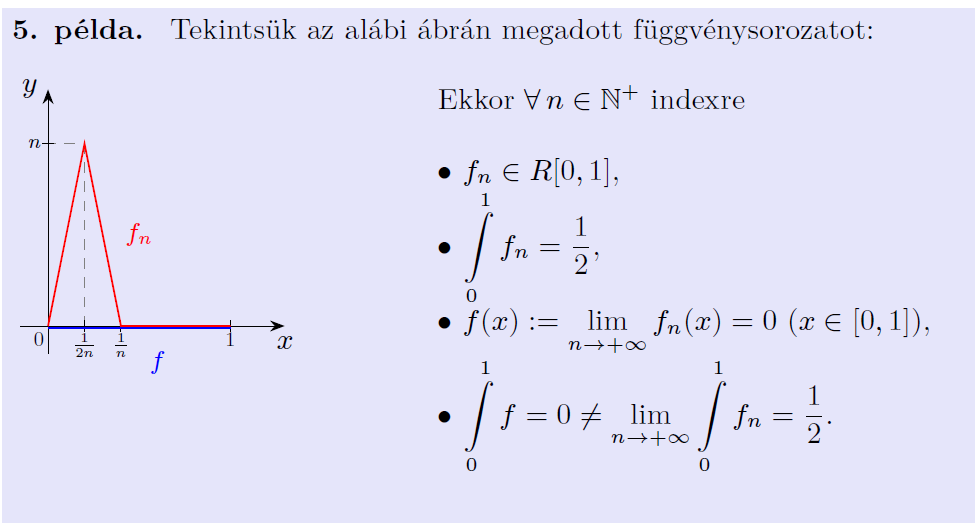
\includegraphics[width=\textwidth]{example1}
\subsection{Mondja ki a határfüggvény integrálhatóságáról szóló tételt!}
\begin{tet}
T.f.h. az $\boxes{a,b} \; \bb{a,b \in \R, \; a< b}$ kompakt intervallumon értelmezett $\fn:\boxes{a,b} \to \R \; \bb{n \in \N}$ függvénysorozatra a következő feltételek teljesülnek:
\begin{itemize}
\item $\fn \in R \boxes{a,b}$ minden $n \in \N$ indexre
\item az $\bb{\fn}$ függvénysorozat az $\boxes{a,b}$ intervallumon egyenletesen tart az $f$ függvényhez.
\end{itemize}
Ekkor 
\begin{enumerate}
\item $f\in R\boxes{a,b}$
\item az integrálok $\bb{\int\limits_a^b \fn} $ sorozata konvergens, és
\[
\int\limits_a^b f = \int\limits_a^b \lim\limits_{n \to +\infty} \fn  = \lim\limits_{n \to +\infty} \int\limits_a^b  \fn
\]
vagyis a limeszképzés és az integrálás műveletei felcserélhetők.
\end{enumerate}
\end{tet}
\subsection{Mondja ki a határfüggvény differenciálhatóságáról szóló tételt!}
\begin{tet}
T.f.h. az $I \subset \R$ korlátos és nyílt intervallumon értelmezett $\fn : I \to \R \; \bb{n\in \N}$ függvénysorozatra a következő feltételek teljesülnek:
\begin{itemize}
\item $\fn \in D\bb{I}$ minden $n \in \N$ indexre
\item az $\bb{\fn'}$ függvénysorozat egyenletesen konvergens $I$-n
\item $\exists a \in I:$ az $\bb{\fn(a)}$ számsorozat konvergens.
\end{itemize}
Ekkor
\begin{enumerate}
\item az $\bb{\fn}$ függvénysorozat egyenletesen konvergens
\item ha $f$ jelöli az $\bb{\fn}$ sorozat határfüggvényét, akkor $f \in D(I)$, és
\[
f' = \bb{\lim\limits_{n \to +\infty}\fn}' = \lim\limits_{n \to +\infty} \fn'
\]
vagyis a limeszképzés és a deriválás műveletei felcserélhetők.
\end{enumerate}
\end{tet}
\end{document}